\renewcommand{\FileName}{logistic}
\begin{frame}
  \frametitle{Logistic regression models}
  \begin{itemize}
	\item{\large\bfseries Response variable}:
      \begin{itemize*}
	   \item Binary response: success/failure, vote: yes/no
	   \item Binomial data: $x$ successes in $n$ trials (grouped data)
	   \item Ordinal response: none, some, severe depression
	   \item Polytomous response: vote Liberal, Tory, Aliance, NDP
      \end{itemize*}
	\item{\large\bfseries Explanatory variables}:
      \begin{itemize*}
	  \item Quantitative regressors: age, dose
	  \item Transformed regressors: $\sqrt{\mathrm{age}}$, log(dose)
	  \item Polynomial regressors: age$^2$, age$^3$, $\cdots$
	  \item Categorical predictors: treatment, sex
	  \item Interaction regessors: treatment $\times$ age, sex $\times$ age
	  \end{itemize*}
  \end{itemize}
\end{frame}

\subsection{Binary response}
\begin{frame}
  \frametitle{Logistic regression models: Binary response}
  \begin{itemize*}
	\item For a binary response, $Y \in (0,1)$, want to predict $\pi = \Pr(Y=1 \given x)$
	\item Linear regression will give predicted values outside $0 \le \pi \le 1$
	\item Logistic model:
	\begin{itemize*}
	  \item $\logit ( \pi_{i}) \equiv \log [ \pi / (1 - \pi)]$ avoids this problem
	  \item logit is interpretable as ``log odds'' that $Y=1$
	\end{itemize*}
	
	\item Probit (normal transform) model $\rightarrow$ similar predictions, but is less
	interpretable
 \begin{center}
  \includegraphics[width=.45\dispwidth,clip]{fig/logitfn}
 \end{center}
  \end{itemize*}

\end{frame}

\begin{frame}
  \frametitle{Logistic regression models: Binary response}
Quantitative predictor: Linear and Logit regression on age
  \begin{itemize*}
	\item Except in extremes, linear
and logistic models give similar predicted values
	\end{itemize*}
\begin{center}
   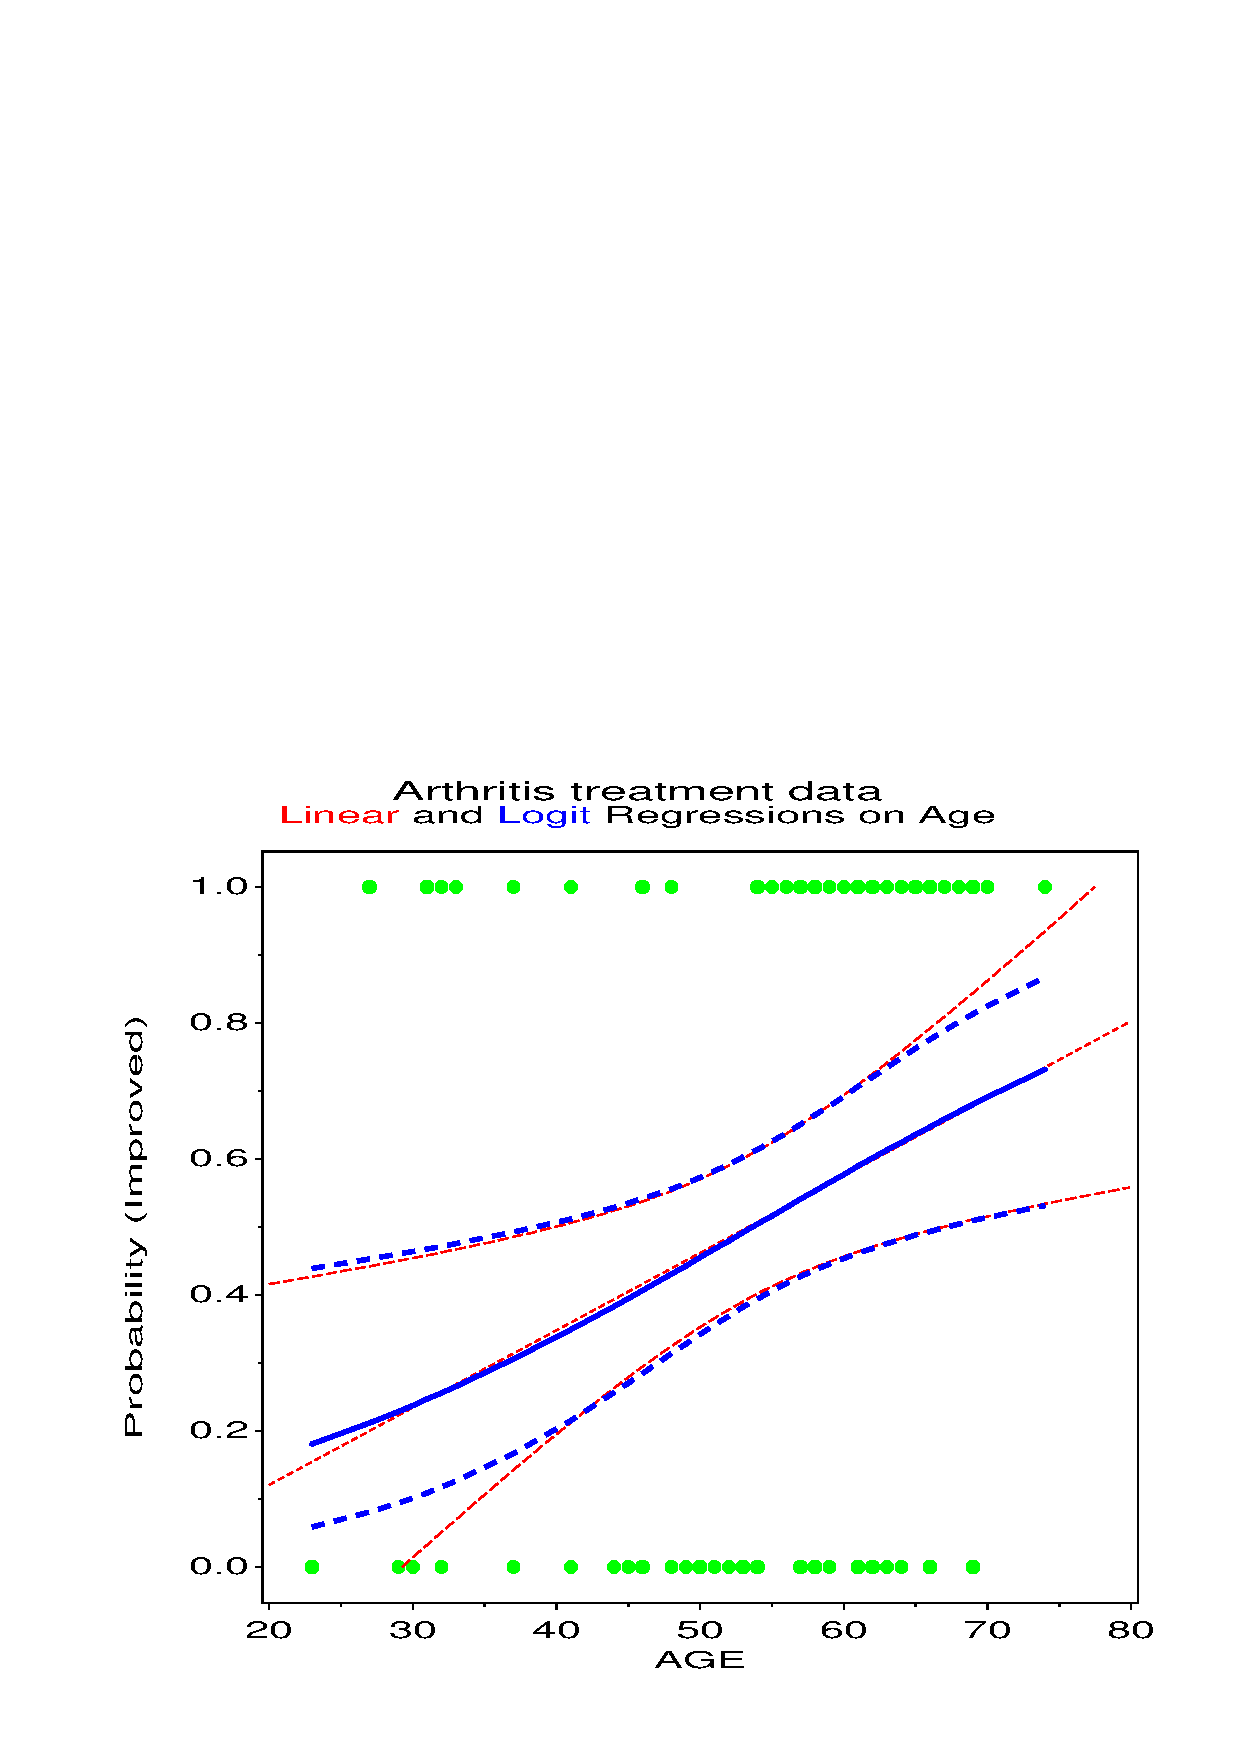
\includegraphics[height=0.7\textheight]{fig/logist1c1}
\end{center}

\end{frame}

\begin{frame}
  \frametitle{Logistic regression models: Binary response}
  \begin{itemize}
	\item For a binary response, $Y \in (0,1)$, 
	let 
	\vec{x} be a vector of $p$ regressors, and  
	$\pi_i$ be the probability, $\Pr (Y=1 \given \vec{x})$. 
	\item The logistic regression
	model is a linear model for the \emph{log odds}, or \emph{logit}
	that $Y=1$, given the values in \vec{x},
\begin{eqnarray*}
  \logit ( \pi_{i}) \equiv \log \left( \frac{\pi_i}{1 - \pi_i}  \right)
   &=& \alpha + \vec{x}_{i}\trans \,  \vec{\beta} \\ % \label{eq:logisr}
   &=& \alpha + \beta_1 x_{i1} + \beta_2 x_{i2} + \cdots + \beta_p x_{ip}
   \nonumber
\end{eqnarray*}
	\item An equivalent (non-linear) form of the model may be specified for
	the probability,  $\pi_i$, itself,
\begin{equation*}
    \pi_i = {\{ 1 + \exp ( -[\alpha + \vec{x}_{i}\trans \,  \vec{\beta} ] ) \}}^{-1}
\end{equation*}

	\item The logistic model is a \emph{linear model} for the log odds, but also a
	\emph{multiplicative} model for the odds of ``success,''
\begin{equation*}
\frac{\pi_i}{1 - \pi_i} = \exp( \alpha + \vec{x}_{i}\trans \,  \vec{\beta} )
   = \exp(\alpha) \exp ( \vec{x}_{i}\trans \,  \vec{\beta} )
\end{equation*}
so, increasing $x_{ij}$ by 1 increases $\logit ( \pi_{i})$ by $\beta_j$,
and multiplies the odds by $e^{\beta_j}$.
%	\item Other ``link functions,'' transforming the probability, $\pi_i$,
%	to the ``linear predictor'' are possible (probit, complementary log-log)   
  \end{itemize}
\end{frame}

\begin{frame}[fragile]
  \frametitle{Logistic regression models: Binary response}
  \begin{itemize}
	\item{\large\bfseries Fitting}: \PROC{LOGISTIC} (or \macro{ROBUST}--- M-estimation)
      \begin{itemize*}
	  \item Data:
    	\begin{itemize*}
		\item Frequency form (from \PROC{FREQ})--- when all predictors are discrete
		\item Case form--- when any predictors are quantitative
		\end{itemize*}
	  \item Models:  
    	\begin{itemize*}
		\item \stmt{CLASS} (V7+)--- no need for dummy variables
    	   \begin{itemize*}
		   \item discrete predictors
		   \item can specify \emph{order} and \emph{parameterization} (effect, polynomial, reference
		   cell)
		   \end{itemize*}
		\item \stmt{MODEL}--- allows \texttt{GLM} syntax, e.g., 

		\verb#model Better = Sex | Treat | Age @2;# 

		\hspace*{5em}$\rightarrow$\texttt{Sex Treat Age Sex*Treat Sex*Age Treat*Age}
		\end{itemize*}
	  \end{itemize*}
  \end{itemize}
\end{frame}

\begin{frame}
  \frametitle{Logistic regression models: Binary response}
  \begin{itemize}
	\item{\large\bfseries Visualization}:
      \begin{itemize*}
	  \item Goal: \emph{see} and \emph{understand} the data and fitted model
	  \item \macro{LOGODDS}: Plot observed responses, fitted and smoothed probabilities
	  \item Model plots:
    	\begin{itemize*}
		\item \stmt{OUTPUT} $\rightarrow$ 
    	   \begin{itemize*}
			\item fitted $\hat{\pi}_i$, lower/upper $(1-\alpha)$ CI, and/or 
			\item fitted logit, $(\alpha + \vec{x}_{i}\trans \,  \hat{\vec{\beta}}) \pm
			z_{1-\alpha/2} se(\logit)$
    	   \end{itemize*}
			
		\item Plot with standard procedures (\PROC{GCHART}, \proc{GPLOT})
		\item Utility macros (\pname{BARS}, \pname{LABEL}, \pname{POINTS}, \pname{PSCALE}, etc.)
		for custom displays
		\end{itemize*}
	  \item Effect plots--- plot hierarchical subset of effects, averaging over
	  those not included.
	  \item \macro{INFLOGIS}: Influence plots for logistic regression models
	  \item \macro{ADDVAR}: Added variable plots for new predictors or transformations of old
%	  \item 
	  \end{itemize*}
  \end{itemize}
\end{frame}

\begin{frame}[fragile]
  \frametitle{Example: Arthritis treatment data}
  \begin{itemize}
  	\item Predictors: Sex, Treatment (treated, placebo), Age
	\item Response: improvement (none, some, marked)
      \begin{itemize*}
	  \item Consider first as binary response: None vs. (Some or Marked)=`Better'
	  \end{itemize*}
	\item Data in case form:
  \end{itemize}
\begin{Input}[fontsize=\small,label=\fbox{\texttt{arthrit.sas}},baselinestretch=0.7]
data arthrit;
   length treat $7. sex $6. ;
   input id treat $ sex $ age improve @@ ;
   case = _n_;
   better  = (improve > 0);  \sascomment{*-- Make binary response;}
datalines ;
57 Treated Male   27 1   9 Placebo Male   37 0
46 Treated Male   29 0  14 Placebo Male   44 0
77 Treated Male   30 0  73 Placebo Male   50 0
  ... (\emph{observations omitted})
56 Treated Female 69 1  42 Placebo Female 66 0
43 Treated Female 70 1  15 Placebo Female 66 1
                        71 Placebo Female 68 1
                         1 Placebo Female 74 2
;
\end{Input}
\end{frame}


\begin{frame}[fragile]
  \frametitle{\macrot{LOGODDS}: Empirical logit plots}
  Problems with visualizing discrete outcomes:
  \begin{itemize}
	\item{\large\bfseries Linearity}: Is a linear relation realistic?
	\item{\large\bfseries Smoothing}: Discrete data often requires smoothing to see!
  \end{itemize}

The \macro{LOGODDS}:
   \begin{itemize*}
   \item Show the data: Plot (0/1) responses [stacked or jittered]
   \item Divide $X$ into groups (e.g., deciles), emprical logit,
   $\log \left(\frac{y_i + 1/2}{n_i - y_i + 1/2}\right)$,
   for each
   \item Linear logistic regression, plus smoothed curve (\macro{LOWESS})
   \end{itemize*}
\vspace{1ex}
\begin{Input}
%include catdata(arthrit);
%logodds(data=arthrit, 
    x=age, y=Better,  \sascomment{/* vars to plot               */}
    smooth=0.5,       \sascomment{/* LOWESS smoothing parameter */}
    plot=logit);      \sascomment{/* plot on logit scale        */}
\end{Input}
\end{frame}

\begin{frame}
\begin{center}
  \includegraphics[width=.9\dispwidth,clip]{fig/logoddt}
\end{center}
\end{frame}

\begin{frame}
\frametitle{Smoothing the binary observations}
Can also use direct smoothing:
\begin{center}
  \includegraphics[width=.8\dispwidth,clip]{fig/arthritis-lowess}
\end{center}
\begin{itemize*}
 \item SAS: \PROC{LOESS}, \macro{lowess}; R: \func{lowess}
 \item There is a hint that the relation may be non-linear
 \item But data is thin at the extremes
\end{itemize*}

\end{frame}


%\endinput

\begin{frame}[fragile]
  \frametitle{\PROC{LOGISTIC}: Model fitting and plotting}
  \begin{itemize}
	\item Specify ordering of response levels (\texttt{order=} or \texttt{descending} options)
	\item Specify parameterizations for \texttt{CLASS} variables
	\item \stmt{OUTPUT} to get fitted logits and probabilities
  \end{itemize}
  \vspace{1ex}
\begin{Input}[label=\fbox{\texttt{glogist1c.sas} $\cdots$},baselinestretch=0.7]
\vspace{.2ex}
proc logistic data=arthrit \sasemph{descending};
   \sasemph{class sex (ref=last) treat (ref=first) / param=ref};
   model better = sex  treat  age;
   \sasemph{output} out=results 
          p=prob l=lower u=upper
          xbeta=logit stdxbeta=selogit / alpha=.33;
\end{Input}
The output includes:
\begin{Output}[gobble=5,fontsize=\small]
                    Type III Analysis of Effects
 
                                     Wald
             Effect      DF    Chi-Square    Pr > ChiSq

             sex          1        6.2576        0.0124
             treat        1       10.7596        0.0010
             age          1        5.5655        0.0183
\end{Output}
\begin{Output}[gobble=1,fontsize=\footnotesize]
             Analysis of Maximum Likelihood Estimates
 
                                  Standard        Wald
 Parameter          DF  Estimate     Error  Chi-Square  Pr > ChiSq

 Intercept           1   -4.5033    1.3074     11.8649      0.0006
 sex       Female    1    1.4878    0.5948      6.2576      0.0124
 treat     Treated   1    1.7598    0.5365     10.7596      0.0010
 age                 1    0.0487    0.0207      5.5655      0.0183

                        Odds Ratio Estimates
                                  
                                   Point          95% Wald
    Effect                      Estimate      Confidence Limits

    sex   Female vs Male           4.427       1.380      14.204
    treat Treated vs Placebo       5.811       2.031      16.632
    age                            1.050       1.008       1.093
\end{Output}
Parameter estimates (reference cell coding):
\begin{itemize*}
  \item $\beta_1 = 1.49 \Rightarrow$ Females $e^{1.49}$=4.43 times more likely to be better than Males
  \item $\beta_2 = 1.76 \Rightarrow$ Treated $e^{1.76}$=5.81 times more likely to be better than Placebo
  \item $\beta_3 = 0.0487 \Rightarrow$ odds ratio=1.05 $\Rightarrow$ odds of improvement
  increase 5\% each year.  Over 10 years, odds of improvement
  $= e^{10 \times 0.0486}= 1.63$, a 63\% increase.  
\end{itemize*}
\end{frame}

\begin{frame}[fragile]
  \frametitle{\PROC{LOGISTIC}: Model plots}
  \begin{itemize}
	\item Plots of fitted values from the \Dset\ specified on the \stmt{OUTPUT}
	\item Plot either predicted probabilities or logits
  \end{itemize}
The first few observations from the \texttt{results} \Dset:
\begin{Output}[gobble=2,fontsize=\footnotesize]
   id sex   treat  age better   prob  lower  upper  logit selogit

   57 Male Treated  27    1    0.194  0.103  0.334 -1.427  0.758 
    9 Male Placebo  37    0    0.063  0.032  0.120 -2.700  0.725 
   46 Male Treated  29    0    0.209  0.115  0.350 -1.330  0.728 
   14 Male Placebo  44    0    0.086  0.047  0.152 -2.358  0.658 
   77 Male Treated  30    0    0.217  0.122  0.357 -1.281  0.713 
   73 Male Placebo  50    0    0.112  0.065  0.188 -2.066  0.622 
    ...
\end{Output}

\end{frame}

\begin{frame}[fragile]
  \frametitle{\PROC{LOGISTIC}: Model plots}
Basic plots:
  \begin{itemize*}
	\item Plot either logit or probability vs. one predictor (continuous or most levels)
	\item Separate curves for one factor
	\item Separate panels for all others (\stmt{BY})
  \end{itemize*}

\begin{listing}
proc gplot data=results;
   plot (logit prob) * age = treat; 
   by sex;
   symbol1 v=circle i=join l=3 c=black;
   symbol2 v=dot    i=join l=1 c=red;
\end{listing}
\end{frame}

\begin{frame}
  \frametitle{\PROC{LOGISTIC}: Model plots}
Enhanced plots:

  \begin{itemize*}
	\item Plot on logit scale, with probability scale at right (\macro{PSCALE})
	\item Show 67\% error bars $\approx \pm 1$ se (\macro{BARS})
	\item Custom legend and panel labels (\macro{LABEL})
  \end{itemize*}

 \begin{center}
  \includegraphics[width=1\dispwidth,clip]{fig/glogist1c}
 \end{center}

\end{frame}

\begin{frame}[fragile]
  \frametitle{\PROC{LOGISTIC}: Model plots}
Enhanced plots:

\begin{Input}[fontsize=\footnotesize,label=\fbox{$\cdots$ \texttt{glogist1c.sas} $\cdots$},baselinestretch=0.7,firstnumber=9]
  \sascomment{*-- Error bars, on logit scale;}
%bars(data=results, var=logit, 
   class=age, cvar=treat, by=age,
   barlen=selogit, \sasemph{out=bars});

  \sascomment{*-- Custom legends and panel labels;}
%label(data=results, y=logit, x=age, xoff=1, cvar=treat,
   by=sex, subset=last.treat, \sasemph{out=label1}, pos=6, text=treat);
%label(data=results, y=2.5, x=20, size=2,
   by=sex, subset=first.sex, \sasemph{out=label2}, pos=6, text=sex);

  \sascomment{*-- Probability scales at right;}		
%pscale(\sasemph{out=pscale}, 
   byvar=sex, byval=%str('Female','Male'));

  \sascomment{*-- Join ANNOTATE datasets;}		
data \sasemph{bars};
   set \sasemph{label1 label2 bars pscale};
proc sort;
   by sex;
\end{Input}
\end{frame}

\begin{frame}[fragile]

\begin{Input}[fontsize=\footnotesize,label=\fbox{$\cdots$ \texttt{glogist1c.sas}},baselinestretch=0.7,firstnumber=30]
title ' '
   h=1.8 a=-90 'Probability Improved'    \sascomment{/* right axis label   */}
   h=2.5 a=-90 ' ';                      \sascomment{/* extra space        */}
goptions hby=0;                          \sascomment{/* suppress BY values */}
proc gplot data=results;
   plot \sasemph{logit * age = treat} / 
         vaxis=axis1 haxis=axis2 hm=1 vm=1
         nolegend \sasemph{anno=bars} frame;
   \sasemph{by sex;}
   axis1 label=(a=90 'Log Odds Improved')
         order=(-3 to 3);
   axis2 order=(20 to 80 by 10) offset=(2,6);
   symbol1 v=+ i=join l=3 c=black;
   symbol2 v=- i=join l=1 c=red;
   label age='Age';
run;
\end{Input}
 \begin{center}
  \includegraphics[width=.7\dispwidth,clip]{fig/glogist1c}
 \end{center}
\end{frame}

\begin{frame}[fragile]
  \frametitle{Models with interactions}
  \begin{itemize}
	\item{\large\bfseries Plotting fitted values}
      \begin{itemize*}
	  \item Only need to change the \stmt{MODEL}
	  \item Output \Dset\ automatically incorporates all model terms
	  \item Plotting steps remain \emph{exactly} the same
    \end{itemize*}
  \end{itemize}
\begin{Input}
proc logistic data=arthrit descending;
   class sex (ref=last) treat (ref=first) / param=ref;
   \sasemph{model  better = sex  treat | age @2};
   output out=results p=prob l=lower u=upper
          xbeta=logit stdxbeta=selogit / alpha=.33;
\end{Input}

 \begin{center}
  \includegraphics[width=.7\dispwidth,clip]{fig/glogist1d}
 \end{center}
\end{frame}

\endinput
% slide template
\begin{frame}
  \frametitle{}
  \begin{itemize}
	\item{\large\bfseries }
      \begin{itemize*}
	  \item 
    	\begin{itemize*}
		\item 
		\item 
		\end{itemize*}
	  \item 
	  \end{itemize*}
	\item{\large\bfseries }
	\item{\large\bfseries }
  \end{itemize}
\end{frame}

